\documentclass[12pt,letterpaper]{article}
\usepackage{graphicx,textcomp}
\usepackage{natbib}
\usepackage{setspace}
\usepackage{fullpage}
\usepackage{color}
\usepackage[reqno]{amsmath}
\usepackage{yhmath}
\usepackage{amsthm}
\usepackage{fancyvrb}
\usepackage{amssymb,enumerate}
\usepackage[all]{xy}
\usepackage{endnotes}
\usepackage{lscape}
\newtheorem{com}{Comment}
\usepackage{float}
\usepackage{hyperref}
\newtheorem{lem} {Lemma}
\newtheorem{prop}{Proposition}
\newtheorem{thm}{Theorem}
\newtheorem{defn}{Definition}
\newtheorem{cor}{Corollary}
\newtheorem{obs}{Observation}
\usepackage[compact]{titlesec}
\usepackage{dcolumn}
\usepackage{tikz}
\usetikzlibrary{arrows}
\usepackage{multirow}
\usepackage{xcolor}
\newcolumntype{.}{D{.}{.}{-1}}
\newcolumntype{d}[1]{D{.}{.}{#1}}
\definecolor{light-gray}{gray}{0.65}
\usepackage{url}
\usepackage{listings}
\usepackage{color}

\definecolor{codegreen}{rgb}{0,0.6,0}
\definecolor{codegray}{rgb}{0.5,0.5,0.5}
\definecolor{codepurple}{rgb}{0.58,0,0.82}
\definecolor{backcolour}{rgb}{0.95,0.95,0.92}

\lstdefinestyle{mystyle}{
	backgroundcolor=\color{backcolour},   
	commentstyle=\color{codegreen},
	keywordstyle=\color{magenta},
	numberstyle=\tiny\color{codegray},
	stringstyle=\color{codepurple},
	basicstyle=\footnotesize,
	breakatwhitespace=false,         
	breaklines=true,                 
	captionpos=b,                    
	keepspaces=true,                 
	numbers=left,                    
	numbersep=5pt,                  
	showspaces=false,                
	showstringspaces=false,
	showtabs=false,                  
	tabsize=2
}
\lstset{style=mystyle}
\newcommand{\Sref}[1]{Section~\ref{#1}}
\newtheorem{hyp}{Hypothesis}

\title{Problem Set 3}

\author{Valeriia Babaian}


\begin{document}
	\maketitle

		\vspace{.25cm}

	\vspace{.5cm}
\section*{Question 1}
\vspace{.25cm}
\noindent We are interested in knowing how the difference in campaign spending between incumbent and challenger affects the incumbent's vote share. 
	\begin{enumerate}
		\item Run a regression where the outcome variable is \texttt{voteshare} and the explanatory variable is \texttt{difflog}.	
		\vspace{.2cm}
		\lstinputlisting[language=R, firstline=38, lastline=38]{PS3 Babaian.R}  
		\item Make a scatterplot of the two variables and add the regression line. 			\vspace{.2cm}
		\lstinputlisting[language=R, firstline=40, lastline=46]{PS3 Babaian.R}  
 \begin{center}
		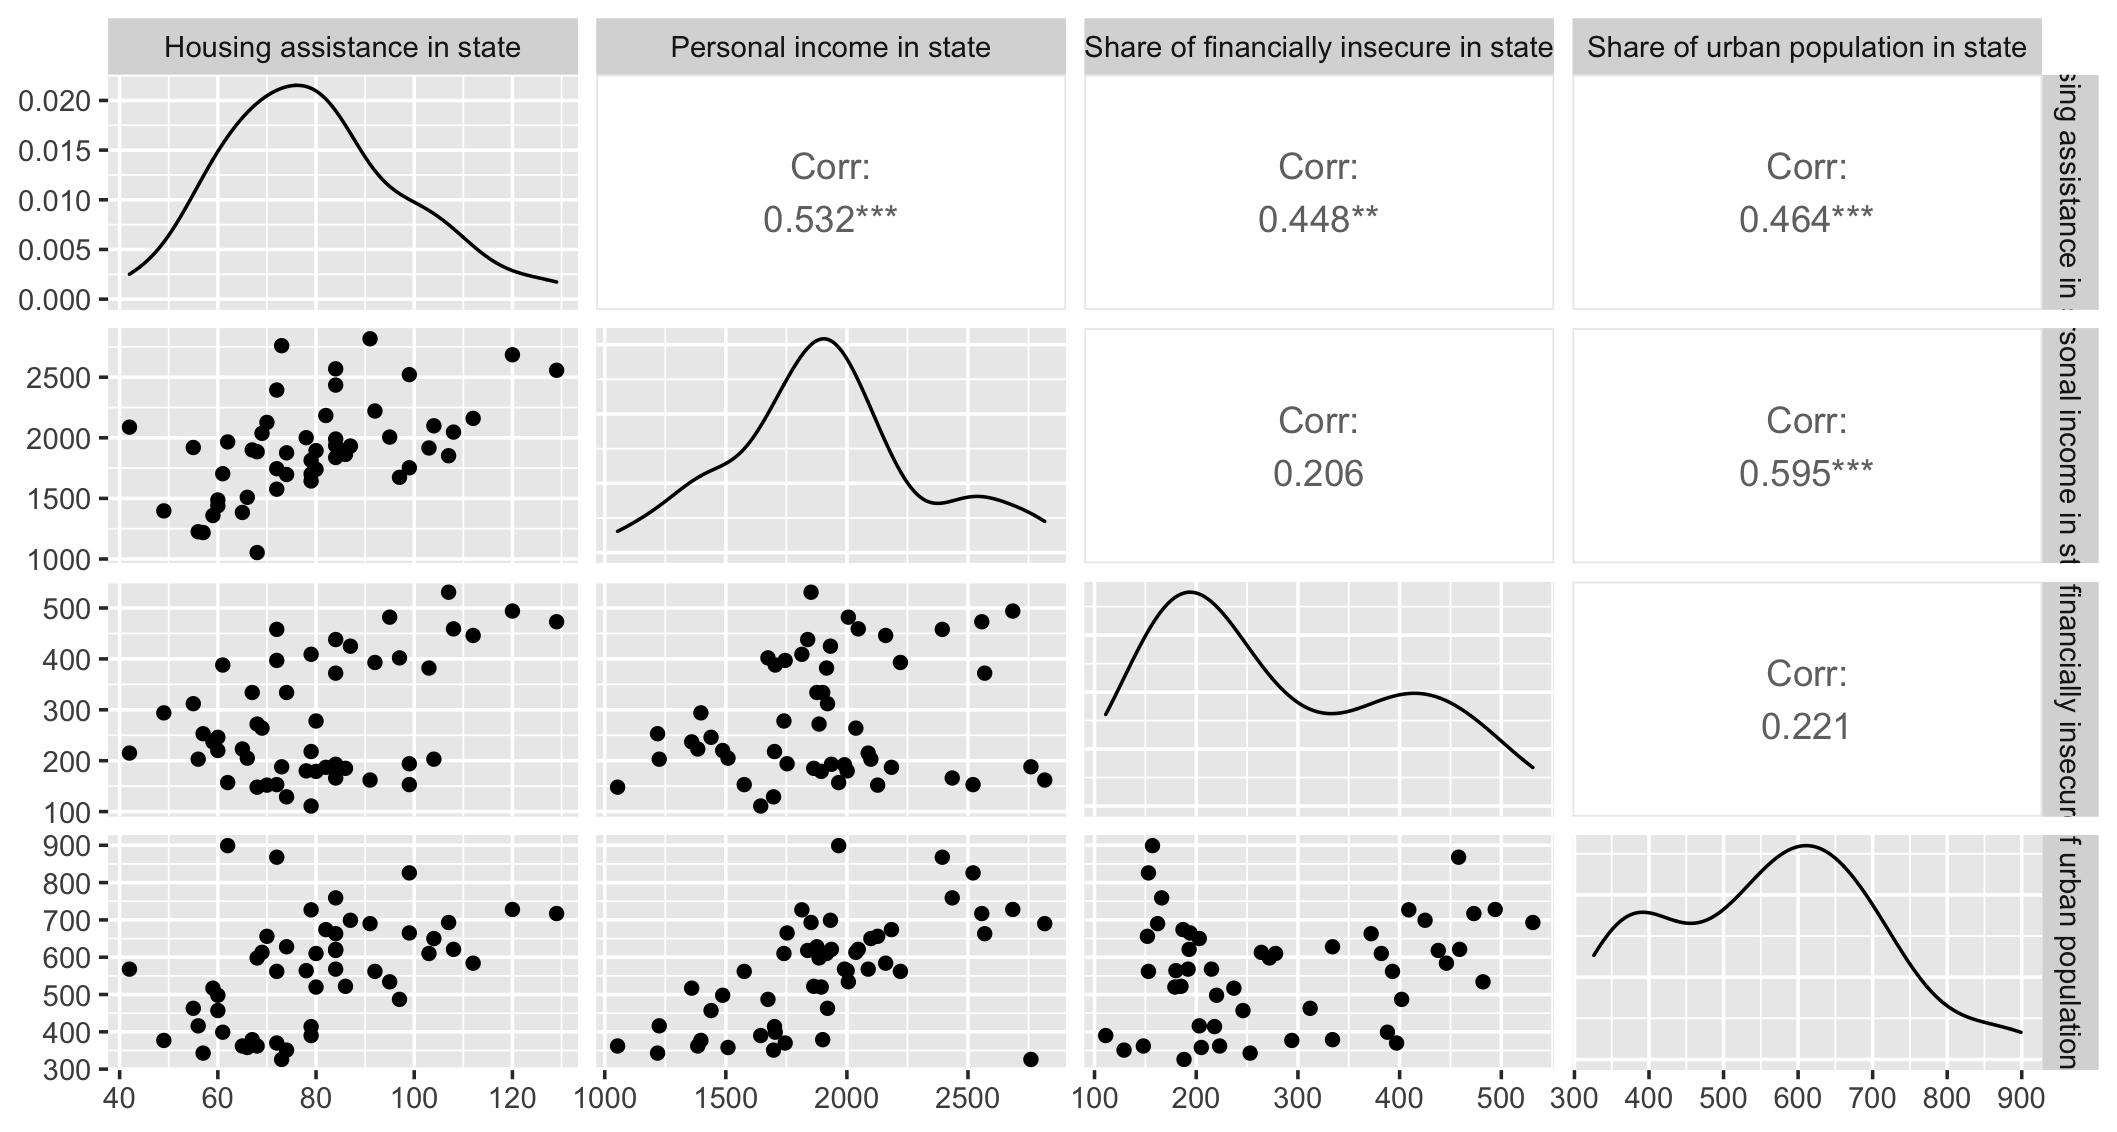
\includegraphics[width=.5\textwidth, height=6.2cm]{Babaian-plot1.png}
	\end{center}
		\item Save the residuals of the model in a separate object.	
			\vspace{.2cm}
		\lstinputlisting[language=R, firstline=48, lastline=48]{PS3 Babaian.R}  
		\item Write the prediction equation.\\
			\lstinputlisting[language=R, firstline=52, lastline=53]{PS3 Babaian.R}  
		\vspace{.2cm}
	
\input{q1.tex}
		Prediction equation: \\
		$\widehat{\textit{voteshare}} = 0.58 + 0.042*\textit{difflog}$
	\end{enumerate}
	
\newpage

\section*{Question 2}
\noindent We are interested in knowing how the difference between incumbent and challenger's spending and the vote share of the presidential candidate of the incumbent's party are related.	\vspace{.25cm}
	\begin{enumerate}
		\item Run a regression where the outcome variable is \texttt{presvote} and the explanatory variable is \texttt{difflog}.	\vspace{.2cm}
			\lstinputlisting[language=R, firstline=60, lastline=60]{PS3 Babaian.R}  
		\item Make a scatterplot of the two variables and add the regression line. 	
		\vspace{.2cm}
		\lstinputlisting[language=R, firstline=62, lastline=69]{PS3 Babaian.R}  
\vspace{.2cm}
\begin{center}
	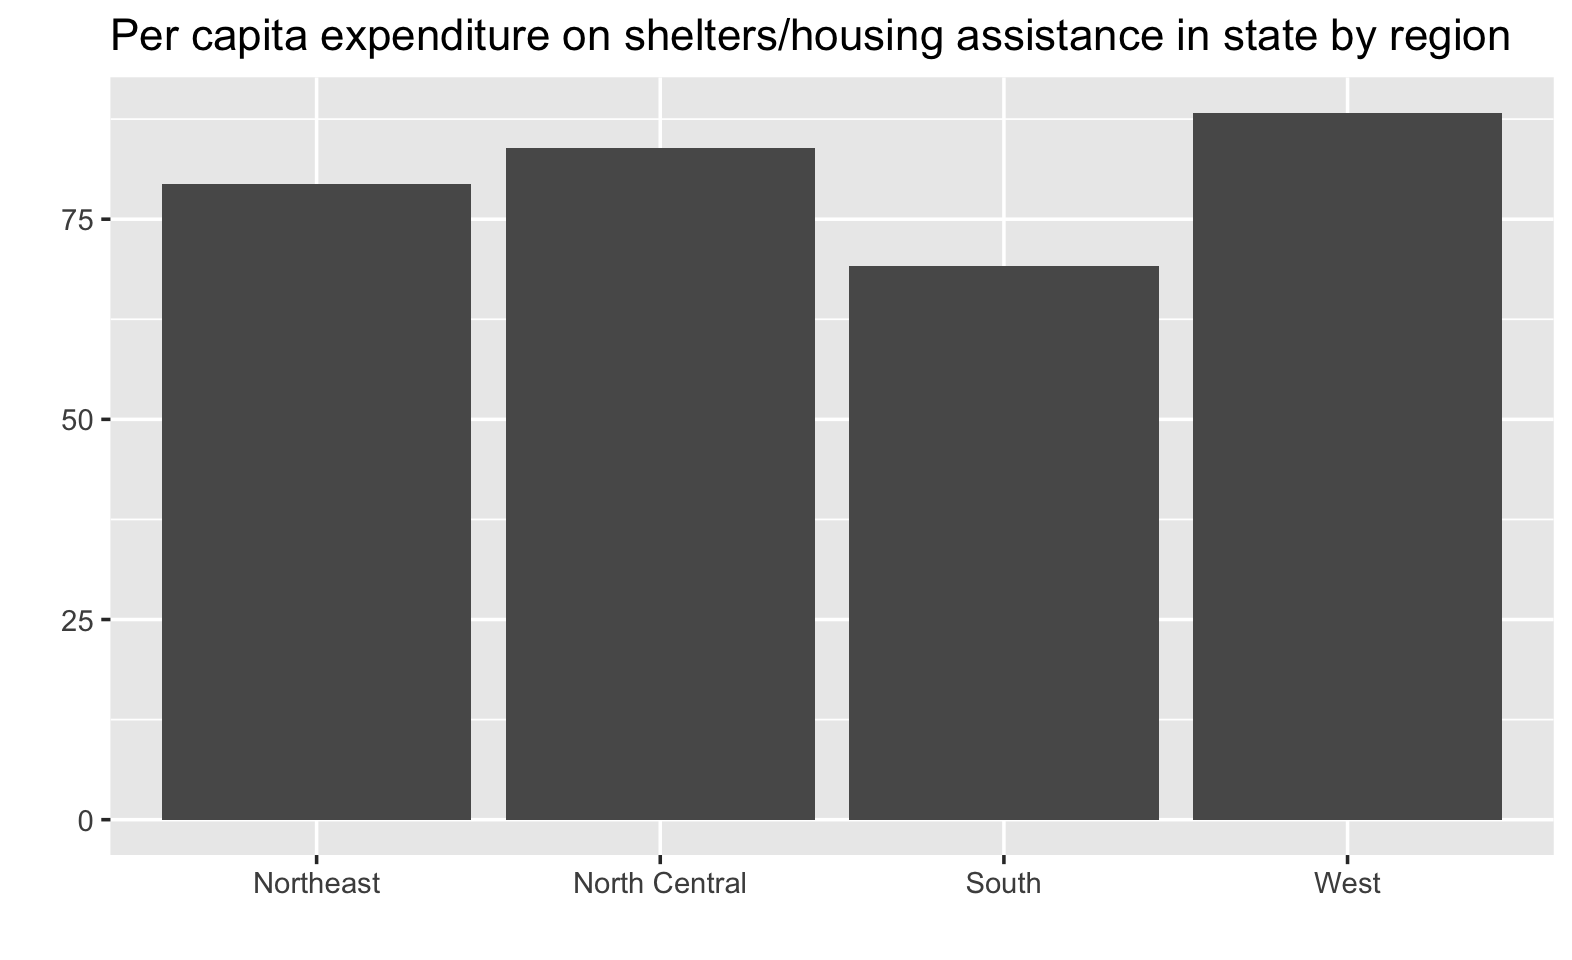
\includegraphics[width=.6\textwidth]{Babaian-plot2.png}
	\end{center}
\vspace{.2cm}
		\item Save the residuals of the model in a separate object.	\vspace{.1cm}
		\vspace{.2cm}
		\lstinputlisting[language=R, firstline=71, lastline=71]{PS3 Babaian.R}  
		\item Write the prediction equation.
			\lstinputlisting[language=R, firstline=74, lastline=75]{PS3 Babaian.R}  
		\input{q2.tex}
		Prediction equation: \\
		$\widehat{\textit{presvote}} = 0.51 + 0.024*\textit{difflog}$
	\end{enumerate}
	
	\newpage	
\section*{Question 3}

\noindent We are interested in knowing how the vote share of the presidential candidate of the incumbent's party is associated with the incumbent's electoral success.
	\vspace{.25cm}
	\begin{enumerate}
		\item Run a regression where the outcome variable is \texttt{voteshare} and the explanatory variable is \texttt{presvote}.
			\vspace{.2cm}
			\vspace{.2cm}
			\lstinputlisting[language=R, firstline=80, lastline=80]{PS3 Babaian.R}  
		\item Make a scatterplot of the two variables and add the regression line. 
		\vspace{.2cm}
		\lstinputlisting[language=R, firstline=82, lastline=89]{PS3 Babaian.R}  
			\vspace{.2cm}
			\begin{center}
				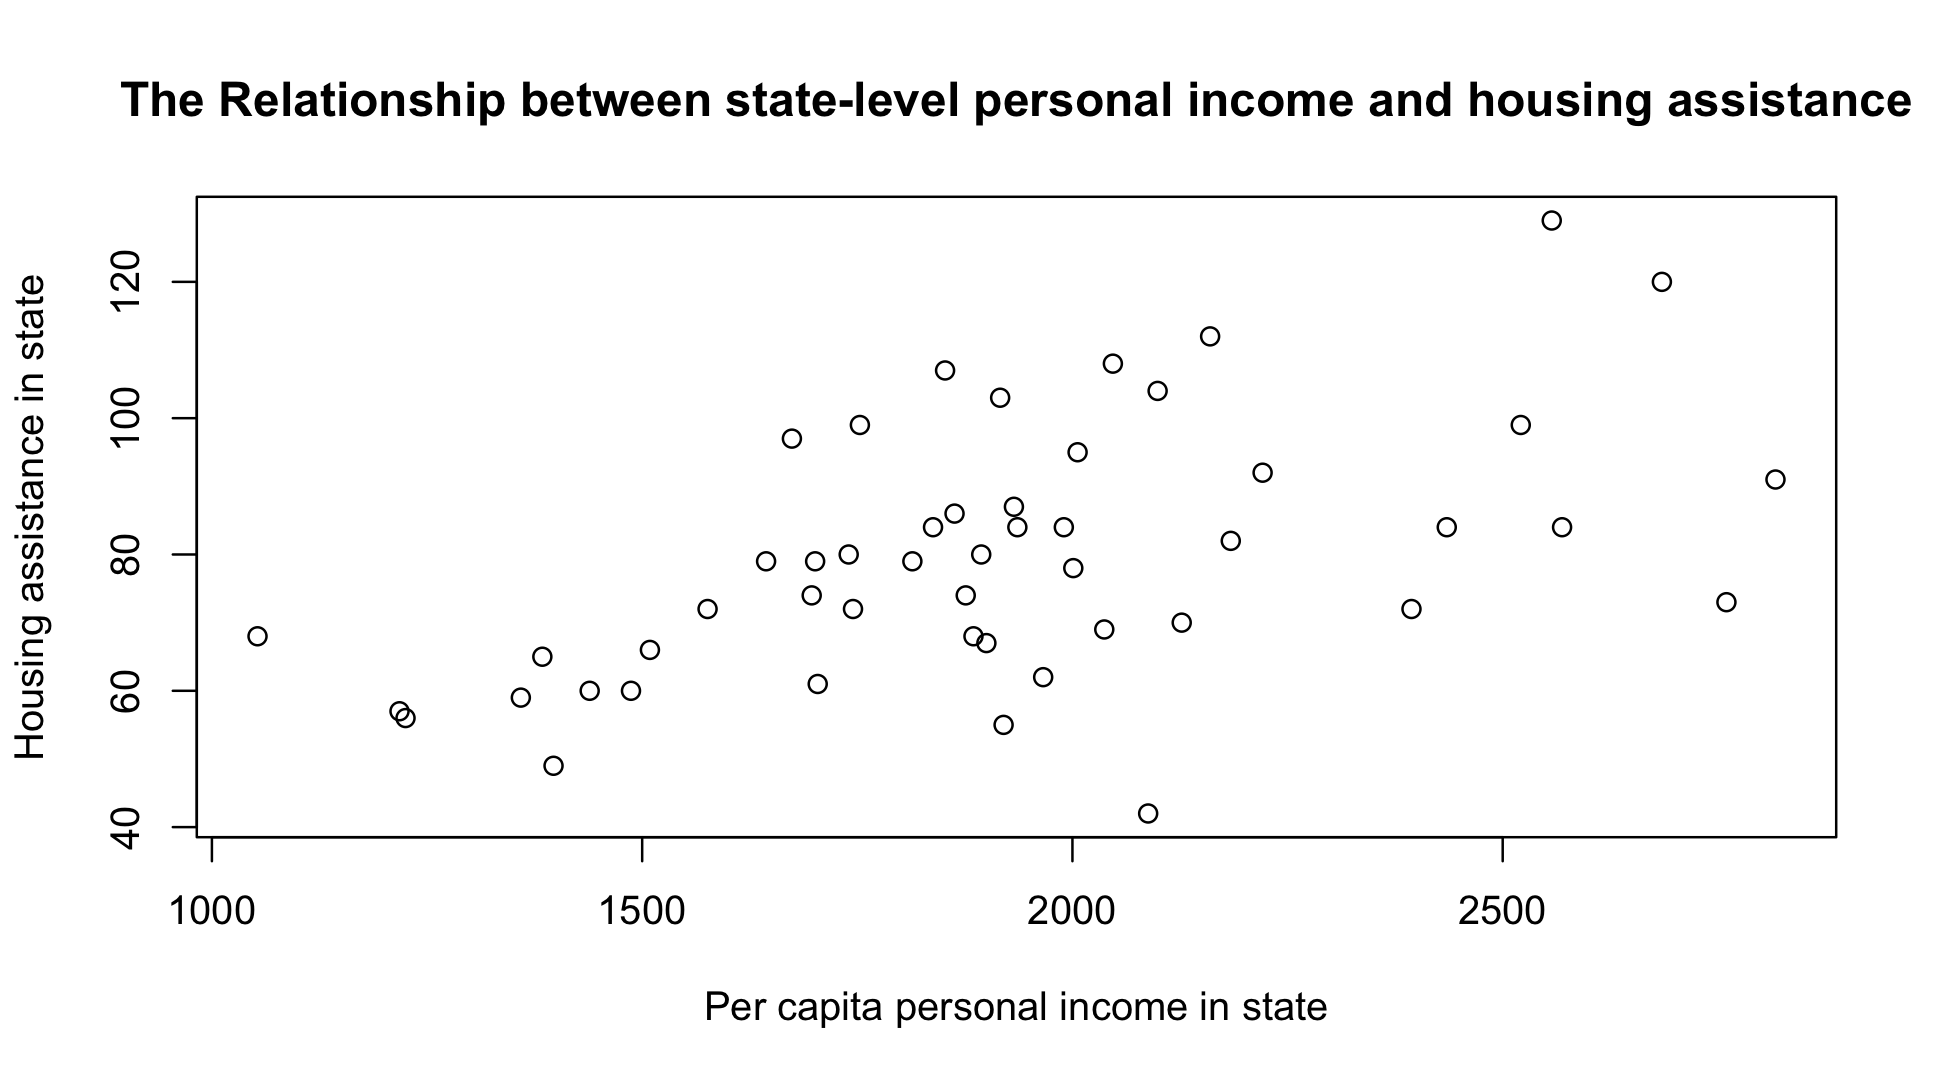
\includegraphics[width=.6\textwidth]{Babaian-plot3.png}
				\end{center}
		\item Write the prediction equation.
			\lstinputlisting[language=R, firstline=91, lastline=92]{PS3 Babaian.R}  
			\input{q3.tex}
		Prediction equation: \\
		$\widehat{\textit{voteshare}} = 0.44 + 0.39*\textit{presvote}$
	\end{enumerate}
	

\newpage	
\section*{Question 4}
\noindent The residuals from part (a) tell us how much of the variation in \texttt{voteshare} is $not$ explained by the difference in spending between incumbent and challenger. The residuals in part (b) tell us how much of the variation in \texttt{presvote} is $not$ explained by the difference in spending between incumbent and challenger in the district.
	\begin{enumerate}
		\item Run a regression where the outcome variable is the residuals from Question 1 and the explanatory variable is the residuals from Question 2.	
			\lstinputlisting[language=R, firstline=97, lastline=97]{PS3 Babaian.R}  
		\item Make a scatterplot of the two residuals and add the regression line. 	\vspace{.2cm}
					\lstinputlisting[language=R, firstline=99, lastline=105]{PS3 Babaian.R}  
					\begin{center}
						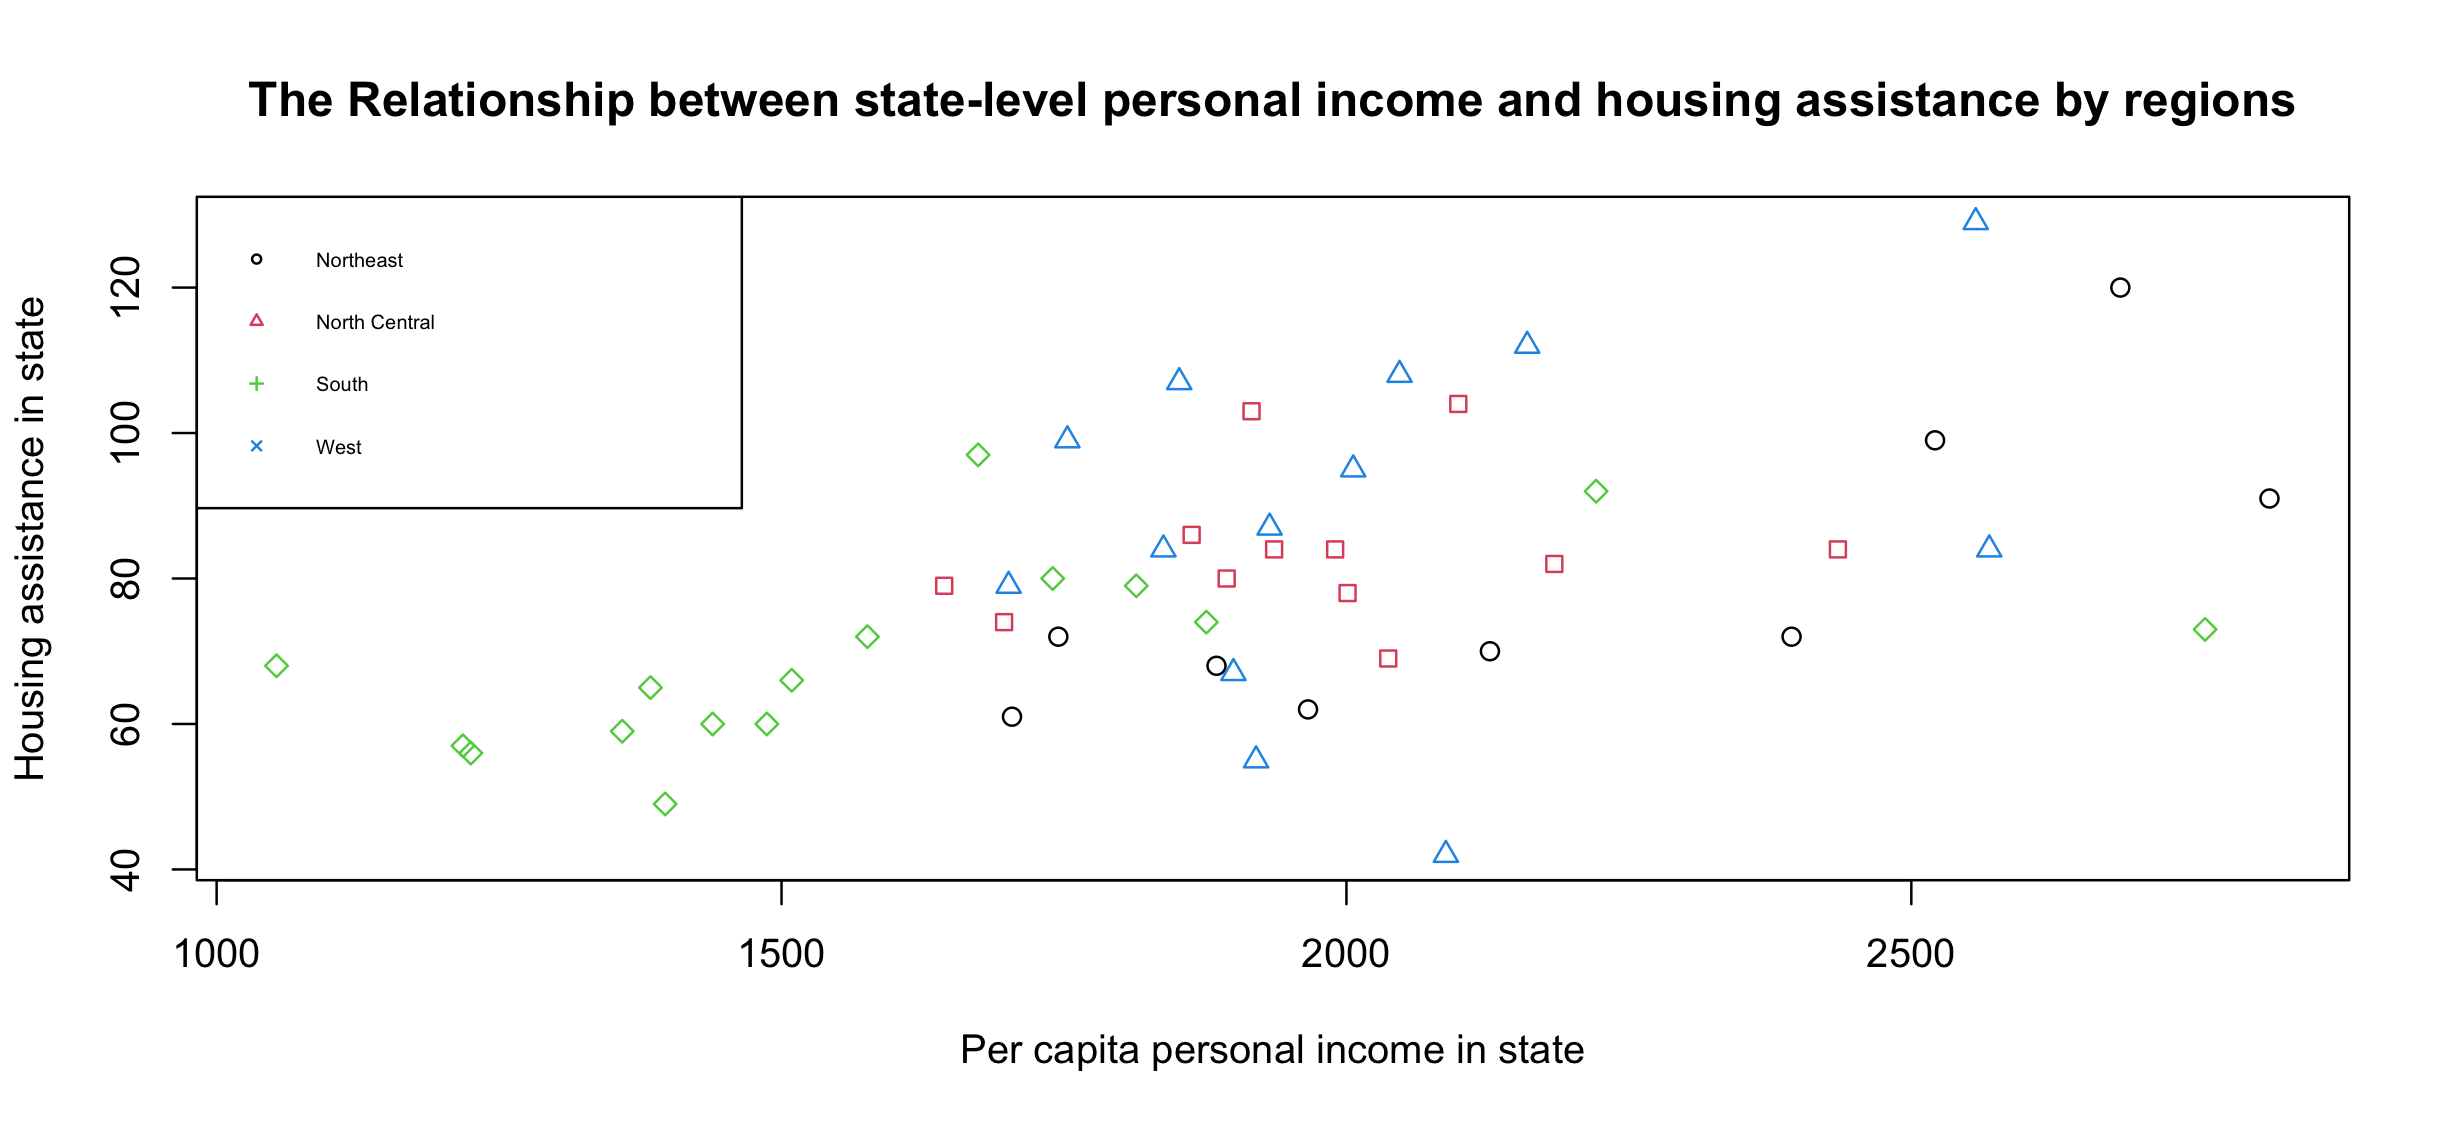
\includegraphics[width=.6\textwidth]{Babaian-plot4.png}
						\end{center}
		\item Write the prediction equation.
							\lstinputlisting[language=R, firstline=109, lastline=110]{PS3 Babaian.R}  
				\input{q4.tex}
			Prediction equation: \\
			$\widehat{\textit{voteshare residuals}} = 0.26*\textit{presvote residuals} - 4.9*10^{-18}$	\\
			(A more precise value of constant is derived from R console output.)			
	\end{enumerate}
	
	\newpage	

\section*{Question 5}
\noindent What if the incumbent's vote share is affected by both the president's popularity and the difference in spending between incumbent and challenger? 
	\begin{enumerate}
		\item Run a regression where the outcome variable is the incumbent's \texttt{voteshare} and the explanatory variables are \texttt{difflog} and \texttt{presvote}.	\vspace{.2cm}
			\lstinputlisting[language=R, firstline=115, lastline=115]{PS3 Babaian.R}  
		\item Write the prediction equation.	\vspace{.2cm}
					\lstinputlisting[language=R, firstline=117, lastline=118]{PS3 Babaian.R}  
						\input{q5.tex}
					Prediction equation: \\
					$\widehat{\textit{voteshare}} = 0.45 + 0.26*\textit{presvote } + 0.036*\textit{difflog}$	\\
		\item What is it in this output that is identical to the output in Question 4? Why do you think this is the case? \\
		The coefficient estimate for \texttt{presvote} is identical to the estimate of its residuals unexplained by \texttt{difflog} for predicting \texttt{voteshare} unexplained by \texttt{difflog}. In this multivariate model (and in any other OLS model), it occurs because total variance is the variance explained by the regression line added residuals. As the residulas of  \texttt{voteshare} and \texttt{presvote} were those left after accounting for  \texttt{difflog}, \texttt{difflog} was already included in the calculation, therefore, the same effect remains true for the effects of observed  \texttt{voteshare} and \texttt{presvote} that can be obtained from the sums of their values predicted by  \texttt{difflog} and their residuals.
	\end{enumerate}




\end{document}
